% IEEE's authorship policy does not allow AI tools to be listed as authors. For an IEEE
% submission, remove Claude from the author block below; the Acknowledgment already
% discloses Claude's part in the experiments, analysis, and writing.
%
% Build: tectonic -X compile main.tex
% Figures: uv run python papers/chestmnist/make_figures.py   (from the repository root)
\documentclass[conference]{IEEEtran}
\usepackage{cite}
\usepackage{amsmath}
\usepackage{graphicx}
\usepackage{booktabs}
\usepackage{array}
\usepackage{url}

\newcommand{\ci}[2]{[#1,\,#2]}

\begin{document}

\title{Candidate Reasons for a Higher ChestMNIST AUROC: How an ImageNet-22k ConvNeXt-Small
Recipe Differs from MedMNIST+}

\author{
\IEEEauthorblockN{Isaiah R. Harville}
\IEEEauthorblockA{Independent Researcher}
\and
\IEEEauthorblockN{Claude}
\IEEEauthorblockA{Anthropic}
}

\maketitle

\begin{abstract}
On native 224-pixel ChestMNIST, the best end-to-end result in the MedMNIST+ benchmark is a
DenseNet-121 with a test macro AUROC of 0.8222, the mean of three seeds. One training run
of our recipe reached 0.8416, with a 95\% bootstrap interval of \ci{0.8369}{0.8461} over
test images. This paper asks which choices in our recipe differ from the MedMNIST+ setup,
since those choices are the candidate reasons for the gap. We compared the two setups from
the MedMNIST+ paper and its released code. Six differences stand out. We used a ConvNeXt-Small
pretrained on ImageNet-22k instead of a DenseNet-121 pretrained on ImageNet-1k. We trained
with random resized crops and small affine jitter, where MedMNIST+ trained without
augmentation. Our cosine schedule decayed the learning rate to $10^{-6}$ over a fixed 10
epochs, while MedMNIST+ used a 100-epoch cosine cycle cut short by early stopping. We
selected the checkpoint on validation AUROC instead of validation loss. We added weight decay
0.05 and stochastic depth 0.2, and we trained in bf16. We ran no ablation, so each difference
is a hypothesis, and we name the experiment that would test it. The result is one seed, the
interval resamples images because MedMNIST has no patient identifiers, and the labels were
mined from radiology reports. Label accuracy at the fixed 0.5 threshold was 0.9470, below
the 0.9474 of a model that predicts every label negative. This is a research model, not a
medical device.
\end{abstract}

\begin{IEEEkeywords}
chest radiograph, multi-label classification, MedMNIST, ChestX-ray14, ConvNeXt, transfer
learning, training recipe, bootstrap confidence interval
\end{IEEEkeywords}

\section{Introduction}

MedMNIST v2 \cite{yang2023medmnist} packages biomedical image datasets as fixed arrays with
fixed splits. Its ChestMNIST subset holds 112,120 frontal chest radiographs from NIH
ChestX-ray14 \cite{wang2017chestxray8}, each with 14 binary finding labels, split
78,468 / 11,219 / 22,433 into training, validation, and test. The MedMNIST+ study
\cite{doerrich2024medmnistplus} benchmarked a range of networks on native 28, 64, 128, and
224-pixel versions of these subsets, with three seeds per setting. For ChestMNIST its best
AUROC is 0.8222 $\pm$ 0.0014, from a DenseNet-121 trained end to end at 224 pixels. That
row is the closest published comparison to our work, because it uses the same native
224-pixel images.

We trained one model on the same images with a recipe written for all MedMNIST 2D subsets,
not tuned for ChestMNIST, and it reached a test macro AUROC of 0.8416, which is 0.019 higher. The question we care about is why. We did not design an
experiment to answer it, so this paper does the next most useful thing. It sets the two
training setups side by side, from the MedMNIST+ paper and its released code
\cite{doerrich2024code}, and for each difference says how plausible it is as a cause and
which ablation would settle it.

Section~\ref{sec:protocol} states the evaluation protocol. Section~\ref{sec:setups} compares
the setups. Section~\ref{sec:results} gives the results against every baseline we track,
and Section~\ref{sec:discussion} discusses the candidate causes and the limits of a single
run.

\section{Data and Evaluation Protocol}
\label{sec:protocol}

We used the ChestMNIST 224-pixel archive of the MedMNIST v3.0 Zenodo release (MD5
\texttt{45bd33e6f06c3e8cdb481c74a89152aa}) through the \texttt{medmnist} 3.0.2 package, with
the official split. The images are single-channel and already 224 $\times$ 224. In the test
split, label prevalence runs from 0.19\% (hernia) to 17.6\% (infiltration), and 94.74\% of
the 314,062 test label decisions are negative.

The labels were not read from the images. Wang et al.\ derived them from the radiology
reports with natural language processing \cite{wang2017chestxray8}, and the test labels come
from the same process. Every number in this paper measures agreement with report-mined
labels.

ChestX-ray14 contains several images of many patients \cite{wang2017chestxray8}, but the
MedMNIST arrays carry no patient identifiers. Our pipeline's check that no patient appears in
two splits could not run, and the run record says so. We cannot rule out patient overlap
between training and test.

The primary metric is test macro AUROC, the unweighted mean of the 14 per-label AUROCs,
computed with scikit-learn \cite{pedregosa2011sklearn} as in the MedMNIST evaluator. Accuracy
(ACC) is the fraction of label decisions that are correct at a fixed 0.5 threshold. Each
metric has a 95\% percentile bootstrap interval from 1,000 replicates with seed 0. Our
pipeline resamples whole patients by default \cite{field2007bootstrapping}. With no patient
identifiers it fell back to resampling single test images, and the metrics file records the
unit as ``sample (no patient IDs)''. The interval covers test-set sampling. It does not cover
variation between training runs.

Model selection used validation data only. The test split was scored once, after selection,
and no threshold or hyperparameter was fitted on it.

\section{Two Training Setups}
\label{sec:setups}

Table~\ref{tab:setups} compares the MedMNIST+ end-to-end setup with ours. For MedMNIST+ we
took each value from the paper's Method section where it is stated there, and otherwise from
\texttt{train.py} and \texttt{config.yaml} in the authors' repository at commit
\texttt{b67b772} \cite{doerrich2024code}. Our values come from the run's resolved
\texttt{config.yaml} and from the script that generates the recipe for all MedMNIST 2D
subsets. That script varies only the epoch count and whether flips are used. ChestMNIST gets
small affine jitter instead of flips, because chest radiographs have a left and a right.

\begin{table*}[t]
\centering
\caption{Training setups compared. MedMNIST+ values are for DenseNet-121 trained end to end
on native 224-pixel ChestMNIST. Source: P is the MedMNIST+ paper
\cite{doerrich2024medmnistplus}, Method section (Model Selection and Training Pipeline);
C is the released code \cite{doerrich2024code}, \texttt{train.py} and \texttt{config.yaml} at
commit \texttt{b67b772}. Our values are from the run's \texttt{config.yaml}.}
\label{tab:setups}
\footnotesize
\renewcommand{\arraystretch}{1.1}
\begin{tabular}{@{}>{\raggedright\arraybackslash}p{2.5cm}
>{\raggedright\arraybackslash}p{5.6cm}
>{\raggedright\arraybackslash}p{6.4cm}
>{\raggedright\arraybackslash}p{1.6cm}@{}}
\toprule
Setting & MedMNIST+ (DenseNet-121) & Ours (ConvNeXt-Small) & Source \\
\midrule
Network & DenseNet-121, timm \texttt{densenet121} & ConvNeXt-Small,
timm \texttt{convnext\_small.fb\_in22k\_ft\_in1k} & P, C \\
Pretraining data & ImageNet-1k & ImageNet-22k, then fine-tuned on ImageNet-1k & P \\
Training scheme & end to end & end to end & P \\
Input at 224 px & native 224; zero padding to 224 is a no-op; gray replicated to 3 channels;
the model's ImageNet mean and std & native 224; 1 channel, timm adapts the stem; mean 0.449,
std 0.226 & P, C \\
Augmentation & none: one deterministic transform for training and validation & random
resized crop (scale 0.7--1.0), rotation $\pm 10^\circ$, translation $\pm 5\%$, no flips &
C \\
Loss & binary cross-entropy with logits & binary cross-entropy with logits; no class weights,
no label smoothing & P, C \\
Optimizer & AdamW, lr $10^{-4}$; weight decay not set (timm default, 0.01 in timm 1.0.31)
& AdamW \cite{loshchilov2019adamw}, lr $10^{-4}$, weight decay 0.05 & P, C \\
Schedule & cosine, one 100-epoch cycle to 0, stepped per epoch & cosine
\cite{loshchilov2017sgdr} over 10 epochs to $10^{-6}$, stepped per epoch & P, C \\
Training length & up to 100 epochs; stop after 5 epochs without a lower validation loss &
fixed 10 epochs (1,227 steps each) & P, C \\
Checkpoint selection & lowest validation loss & highest validation macro AUROC & C \\
Batch size & 64 & 64 & P \\
Regularization & none set & stochastic depth 0.2 \cite{huang2016stochastic} & C \\
Weight averaging & none & EMA, decay 0.99919; used only to choose the epoch
(Section~\ref{sec:ema}) & C \\
Numeric precision & fp32 (no autocast in the code) & bf16 mixed & C \\
Seeds & 3 & 1 (seed 0) & P \\
GPU & NVIDIA RTX A5000 & NVIDIA GeForce RTX 4070 Ti & P \\
\bottomrule
\end{tabular}
\end{table*}

Two rows need a note. MedMNIST+ zero-pads lower resolutions to 224 pixels, but at 224 the
padding is zero pixels wide, so both setups see the same native images. Their code loads the
grayscale images as three identical channels. timm adapts our pretrained RGB stem to one
channel by summing its weights over the color channels \cite{wightman2019timm}. Because the
first convolution is linear, the two are the same function at initialization; only the
normalization constants differ.

\subsection{Which weights were evaluated}
\label{sec:ema}
Lightning's EMA callback swaps the averaged weights in for each validation pass, so the
per-epoch validation AUROC that drove selection was measured on the EMA weights. The
checkpoint, however, was saved in weights-only mode, and in that mode Lightning skips the
hook that writes the averaged weights into the file. The saved checkpoint holds the raw
weights from the selected epoch. We confirmed this with a small script on the same Lightning
version (2.6.6). Every test number in this paper comes from those raw weights. EMA affected
only which epoch was chosen. On validation the raw weights scored 0.8470, against 0.8512 for
the EMA weights of the same epoch (Fig.~\ref{fig:curves}). We did not score the EMA weights
on test, because choosing between the two after seeing test results would make the test
split a second selection step.

\section{Results}
\label{sec:results}

Training ran for 53 minutes on one GPU in PyTorch \cite{paszke2019pytorch} and PyTorch
Lightning \cite{falcon2019lightning}. Fig.~\ref{fig:curves} shows the per-epoch log.
Training loss fell every epoch, from 0.1626 to 0.1146. Validation AUROC of the EMA weights
reached 0.8512 at epochs 6 and 7 (0.85118 and 0.85119) and fell to 0.8441 by epoch 10.
Selection picked epoch 7.

\begin{figure}[t]
\centering
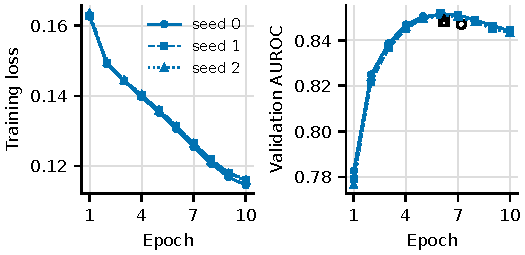
\includegraphics[width=\columnwidth]{figures/training_curves.pdf}
\caption{Training loss (top) and validation macro AUROC (bottom) per epoch. The line is the
AUROC of the EMA weights, logged during training. The diamond is the saved raw weights,
rescored after training. The dashed line marks the selected epoch.}
\label{fig:curves}
\end{figure}

Table~\ref{tab:main} places the test result against every baseline in the project's
baseline file. Our macro AUROC is 0.8416 \ci{0.8369}{0.8461}, and all ten published values
lie below the lower end of the interval. The MedMNIST+ DenseNet-121 is 0.0194 below our
point estimate. MedViTV2-L \cite{manzari2025medvitv2}, at 0.823, is the highest published
value. It trains on 28-pixel images upscaled to 224 and does not say how many runs it
summarizes. C-Mixer \cite{zheng2023cmixer}, a preprint that is not in our baseline file,
reports 0.822 at 28 pixels, also below our interval.

\begin{table*}[t]
\centering
\caption{ChestMNIST test results. AUROC is the macro mean over 14 labels; ACC is label
accuracy at a 0.5 threshold. Our intervals are 95\% percentile bootstrap intervals over test
images. ``28$\rightarrow$224'' means 28-pixel images upscaled to 224.}
\label{tab:main}
\footnotesize
\begin{tabular}{@{}llllll@{}}
\toprule
Method & Input & Runs & AUROC & ACC & Source \\
\midrule
ConvNeXt-Small (ours) & native 224 & 1 & \textbf{0.8416} \ci{0.8369}{0.8461} & 0.9470 \ci{0.9461}{0.9479} & this work \\
MedViTV2-L & 28$\rightarrow$224 & not stated & 0.823 & 0.967 & \cite{manzari2025medvitv2}, Table 5 \\
DenseNet-121 (MedMNIST+) & native 224 & mean of 3 & 0.8222 & 0.9484 & \cite{doerrich2024medmnistplus}, Supp.\ Table S3 \\
MedViT-L & 28$\rightarrow$224 & not stated & 0.805 & 0.959 & \cite{manzari2023medvit}, Table 3 \\
Google AutoML Vision & 28 & $\geq 3$ & 0.778 & 0.948 & \cite{yang2023medmnist}, Table 3 \\
ResNet-18 & 28$\rightarrow$224 & $\geq 3$ & 0.773 & 0.947 & \cite{yang2023medmnist}, Table 3 \\
ResNet-50 & 28$\rightarrow$224 & $\geq 3$ & 0.773 & 0.948 & \cite{yang2023medmnist}, Table 3 \\
ResNet-50 & 28 & $\geq 3$ & 0.769 & 0.947 & \cite{yang2023medmnist}, Table 3 \\
ResNet-18 & 28 & $\geq 3$ & 0.768 & 0.947 & \cite{yang2023medmnist}, Table 3 \\
AutoKeras & 28 & $\geq 3$ & 0.742 & 0.937 & \cite{yang2023medmnist}, Table 3 \\
auto-sklearn & 28 & $\geq 3$ & 0.649 & 0.779 & \cite{yang2023medmnist}, Table 3 \\
\midrule
Predict no finding for every label & -- & -- & 0.5 & 0.9474 & computed \\
\bottomrule
\end{tabular}
\end{table*}

Accuracy does not improve. Ours is 0.9470 \ci{0.9461}{0.9479}, below the MedMNIST+
DenseNet-121 (0.9484) and MedViTV2-L (0.967), with an upper bound below both. It is also
below 0.9474, the accuracy of predicting every label negative, which we computed from the
test labels. At the 0.5 threshold the model marks 2.24\% of label decisions positive, while
5.26\% are positive in the labels. The protocol fixes the threshold, so we did not tune it,
and we make no accuracy claim.

\section{Discussion}
\label{sec:discussion}

\subsection{Candidate causes of the AUROC gap}
Every row of Table~\ref{tab:setups} except the loss, the batch size, and the training scheme
differs, and we changed them all at once. The paragraphs below rank the differences by how
plausible we find them. Each is a hypothesis. None has been tested.

\emph{Backbone and pretraining data.} ConvNeXt \cite{liu2022convnext} is a newer
architecture than DenseNet-121, and our weights saw ImageNet-22k before ImageNet-1k. Both
changes give a better starting representation for natural images, and we expect them to
account for part of the gap. The test is to rerun our recipe twice, once with the
ImageNet-1k-only ConvNeXt-Small weights and once with DenseNet-121, holding everything else
fixed. The first run separates pretraining data from architecture, and the second puts the
MedMNIST+ network inside our recipe.

\emph{Learning-rate schedule and training length.} Fig.~\ref{fig:lr} shows the two schedules.
Ours fell to $3.5 \times 10^{-5}$ by the selected epoch. The MedMNIST+ cycle spans 100
epochs, so at epoch 10 its rate is still about $0.98 \times 10^{-4}$, and early stopping can
end training before the rate has decayed much. We do not know at which epoch their ChestMNIST
runs stopped. If they stopped early, their models were selected from a phase of training with
a near-constant high learning rate, while ours was selected late in an annealed run. The test is
to run our recipe with their schedule and stopping rule, and theirs with a 10-epoch cosine.

\begin{figure}[t]
\centering
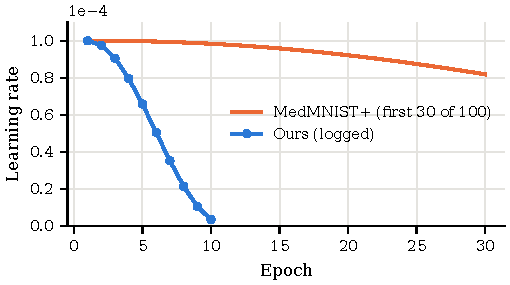
\includegraphics[width=\columnwidth]{figures/lr_schedules.pdf}
\caption{Learning rate by epoch. Ours is the logged value. The MedMNIST+ curve is
recomputed from the released code: timm's cosine scheduler with a 100-epoch cycle, stepped
once per epoch. It is shown for its first 30 epochs.}
\label{fig:lr}
\end{figure}

\emph{Selection metric.} We kept the epoch with the best validation AUROC. MedMNIST+ keeps
the epoch with the lowest validation loss. On a label matrix that is 95\% negative, the
binary cross-entropy is dominated by easy negatives and can reach its minimum at a different
epoch than macro AUROC, which weights each label equally. Selecting on the reported metric
should favor that metric. Our log does not record validation loss, so we cannot check where
it bottomed out in our run. The test is to log validation loss and compare the epochs the two
rules pick. That needs one rerun that keeps every epoch's checkpoint, but no change to the
recipe.

\emph{Augmentation.} MedMNIST+ trains on the unaltered images, while we used random resized
crops and small rotations and translations. With 78,468 training images and 10 epochs, the
effect could go either way. The test is to train our recipe without augmentation.

\emph{Regularization.} We used weight decay 0.05 against the timm default of 0.01, and
stochastic depth 0.2 against none. Over 10 epochs we expect a small effect, but we have
not measured it. The test is to set both to the MedMNIST+ values.

\emph{Differences we consider unlikely causes.} Mixed precision changes arithmetic, not the
model, and we do not expect bf16 to raise AUROC. The one-channel stem and the
three-channel input are the same function at initialization. EMA cannot explain the reported
number, because the reported weights are the raw weights (Section~\ref{sec:ema}); at most it
changed which epoch was chosen, and the EMA curve was nearly flat between epochs 5 and 7.
The test for EMA is to select on the raw weights' validation AUROC.

A credible ablation would change one factor at a time and repeat each setting with at least
three seeds, so that its spread can be compared with the 0.0014 seed standard deviation that
MedMNIST+ reports for DenseNet-121. Our repository includes a paired bootstrap over shared
test images for comparing two runs, which suits this design.

\subsection{Limitations}
\emph{One seed.} Every number comes from one run with seed 0. GPU training allowed
nondeterministic kernels, so a rerun will not reproduce the weights bit for bit. Seed
variance is the largest uncertainty our interval leaves out. Our point estimate is above the
MedMNIST+ mean by 14 of their seed standard deviations, but we have no estimate of our own.

\emph{Image-level bootstrap.} If patients repeat within the test split, the image-level
interval is too narrow, by an amount we cannot estimate. Its lower half-width is 0.0047. It
would have to grow about four-fold before it reached 0.823. Patient overlap between training
and test, which we also could not check, would affect our model and the baselines alike.

\emph{Report-mined labels.} Errors in the NLP-derived labels limit the AUROC any model can
reach against them and may reward fitting the labeling process. We did not evaluate on
radiologist-read labels, so we cannot say whether the gap survives a better reference
standard.

\emph{Accuracy and scope.} The model does not improve accuracy at the fixed threshold and
scores below the all-negative predictor on it. All data comes from one source dataset at
reduced resolution. This is a research model. It is not a medical device and must not be
used for diagnosis.

\section{Reproducibility}
\label{sec:repro}
The model trained at commit \texttt{ab39eb9758be4bb65d09}\allowbreak\texttt{1fad1d98b521edfbf837}
of \url{https://github.com/isaiah-harville/opendiagnostics}, with a clean working tree, by
\begin{center}
\footnotesize
\texttt{uv run opendiagnostics fit -c}\\
\texttt{models/chestmnist-convnext/config.yaml}
\end{center}
on Windows 11 with an NVIDIA GeForce RTX 4070 Ti, CUDA 13.2, Python 3.12.16, PyTorch 2.15.0,
torchvision 0.29.2, Lightning 2.6.6, timm 1.0.31, and torchmetrics 1.9.0. The model has
49,462,382 parameters. The checkpoint was rescored with the code at commit
\texttt{8496d9cfc6132ce66293}\allowbreak\texttt{7ff05c755f0f2fad972c}, which fixed how the
run's configuration records one augmentation argument; the numbers here come from that
rescoring. The run directory \texttt{models/chestmnist-convnext/runs/}\allowbreak
\texttt{20261126-165951-ab39eb97} holds the resolved configuration, the per-epoch log, the
metrics, and per-image probabilities for every validation and test image, so every AUROC and
interval here can be recomputed without the model. The 198~MB checkpoint is public at
\url{https://diagnostics.harville.dev/opendiagnostics-weights/chestmnist-convnext/20261126-165951-ab39eb97/checkpoint.ckpt}
with SHA-256 \texttt{b932b25e691820f2}\allowbreak\texttt{9101d7fd656275ea}\allowbreak
\texttt{f72323dee6903a4f}\allowbreak\texttt{b41e2d6916b8e}. The figures are drawn by
\texttt{papers/chestmnist/make\_figures.py} from the committed run files.

\section{Conclusion}
A single run of a recipe that was not tuned for ChestMNIST scored above the published
AUROCs we could source, and it differs from the MedMNIST+ setup in at least six ways. The
comparison narrows the search but does not finish it. The cheapest next step is the
selection-metric check, which needs one rerun that keeps every epoch's checkpoint. The most informative is a
one-factor ablation of pretraining data and schedule over three seeds. Until those runs
exist, the gap should be read as a property of the whole recipe, not of any one choice.

\section*{Acknowledgment}
Claude, an AI model made by Anthropic, took part in the experiments, the analysis, and
the writing of this paper.

\bibliographystyle{IEEEtran}
\bibliography{refs}

\end{document}
